\documentclass[tikz,border=10pt]{standalone}
\usepackage{mathabx}
\usetikzlibrary{backgrounds}
\usepackage{newunicodechar}
\newunicodechar{♮}{$\natural$}
\newunicodechar{♭}{$\flat$}
\newunicodechar{♯}{$\sharp$}
\newunicodechar{➚}{$\nearrow$}
\newunicodechar{➘}{$\searrow$}
\newunicodechar{Ȧ}{\stackon[0.8pt]{A}{.}}
\newunicodechar{Ḃ}{\stackon[0.8pt]{B}{.}}
\newunicodechar{Ċ}{\stackon[0.8pt]{C}{.}}
\newunicodechar{Ḋ}{\stackon[0.8pt]{D}{.}}
\newunicodechar{Ė}{\stackon[0.8pt]{E}{.}}
\newunicodechar{Ḟ}{\stackon[0.8pt]{F}{.}}
\newunicodechar{Ġ}{\stackon[0.8pt]{G}{.}}


\def\centerarc[#1](#2)(#3:#4:#5);%
{
  \draw[#1]([shift=(#3:#5)]#2) arc (#3:#4:#5);
}


\begin{document}
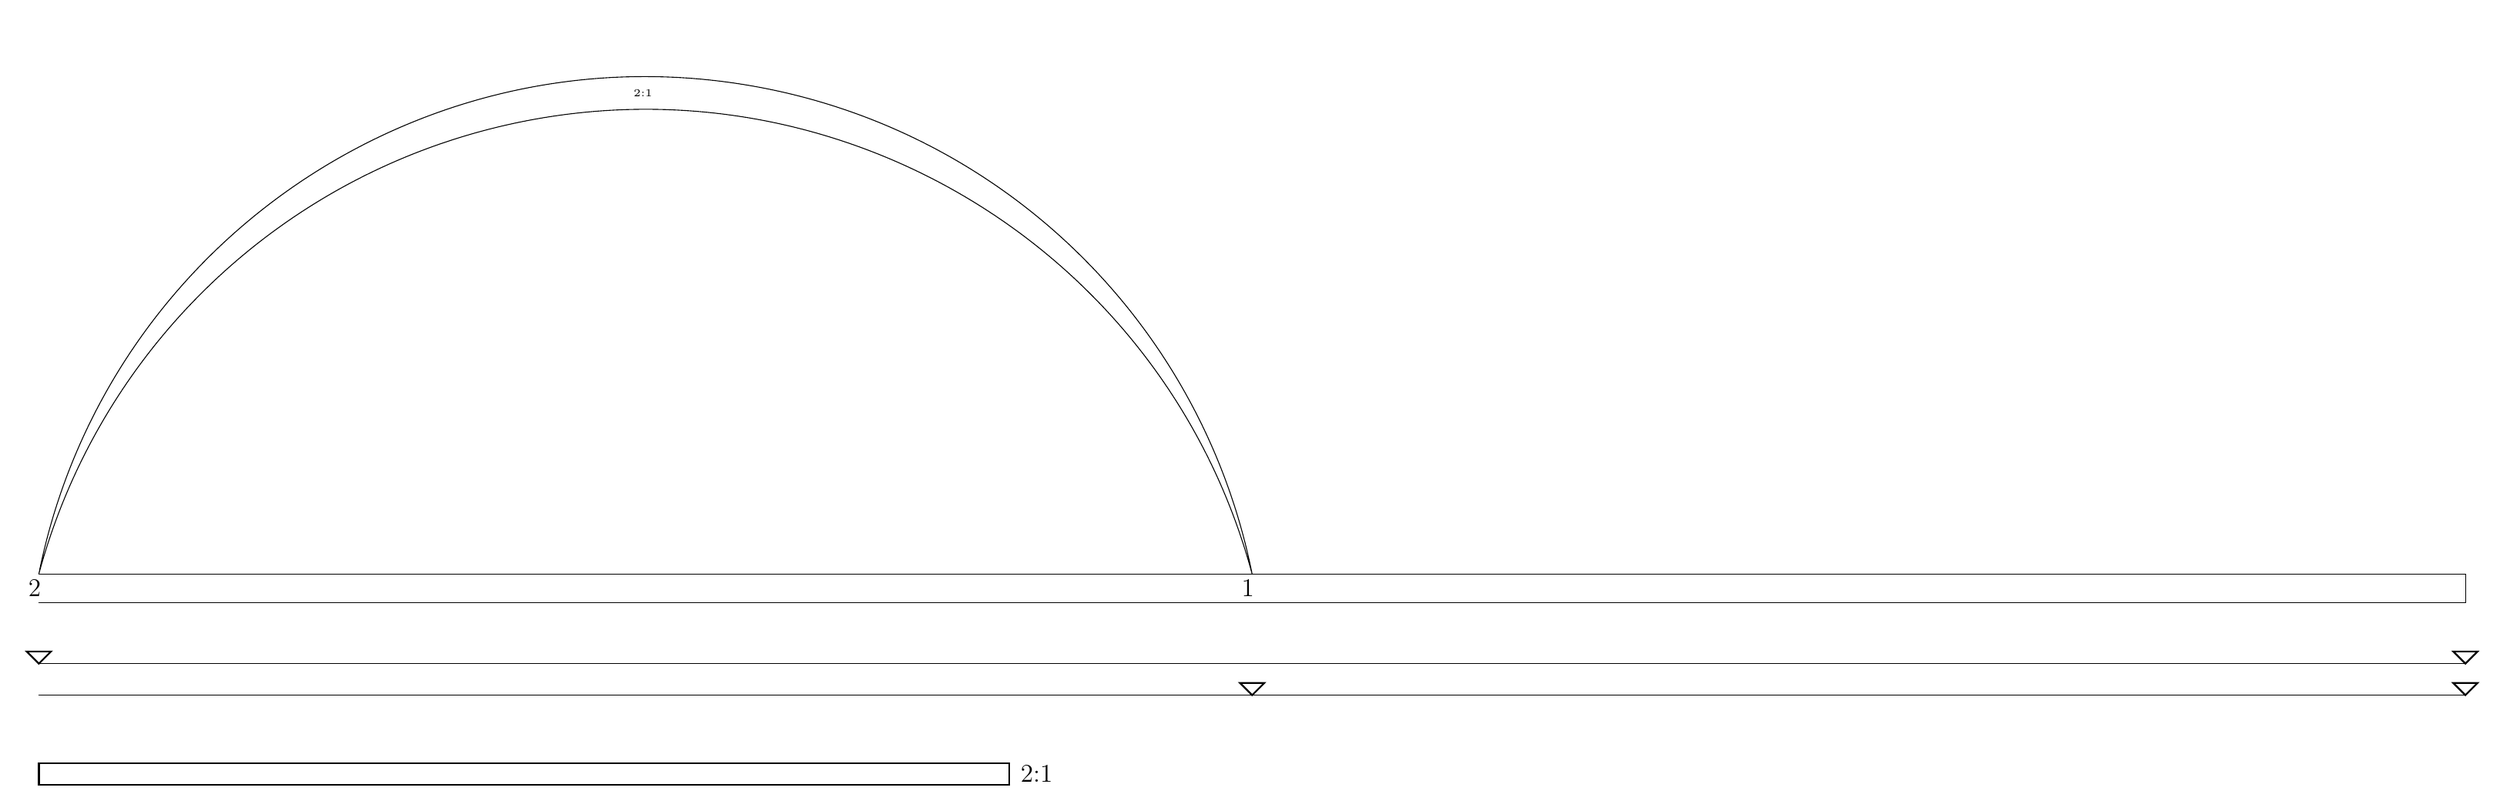
\begin{tikzpicture}

\draw (0.0,0.0) -- (40.0,0.0);
\draw (0.0,-0.48000002) -- (40.0,-0.48000002);
\draw (40.0,-0.48000002) -- (40.0,0.0);
\draw[fill=white] (0.0,0.0) arc[start angle=168.69007234725063, end angle=11.309932661705695, radius=10.198039] arc[start angle=15.10957543472025, end angle=164.89041932895233, radius=10.3580885] -- cycle;
\node[align=center] at (10.0,7.928064) { \tiny 2:1 };
\node[align=center] at (0.0, -0.24000001) { \large 2 };
\node[align=center] at (20.0, -0.24000001) { \large 1 };
\draw (0.0,-1.48) -- (40.0,-1.48);
\draw[thick] (0.0, -1.48) -- (0.2, -1.2800001) -- (-0.2, -1.2800001) --  cycle;
\draw[thick] (40.0, -1.48) -- (40.2, -1.2800001) -- (39.8, -1.2800001) --  cycle;
\draw (0.0,-2.0) -- (40.0,-2.0);
\draw[thick] (20.0, -2.0) -- (20.2, -1.8000001) -- (19.800001, -1.8000001) --  cycle;
\draw[thick] (40.0, -2.0) -- (40.2, -1.8000001) -- (39.8, -1.8000001) --  cycle;
\draw[thick] (0.0, -3.12) -- (15.999503, -3.12) -- (15.999503, -3.48) -- (0.0, -3.48) --  cycle;
\node[anchor=west] at (16.059504, -3.3) { \large 2:1 };
\end{tikzpicture}
\end{document}